
\msection{Distributed Processing (Objective 1)}
\label{sec:aim1}

Recent work in machine learning has studied the effect of
communication constraints and parallelization in distributed
estimation. There is a close parallel in vision, where any given input
is sensed by multiple parts of the retina and an accurate percept
needs to be constructed.

\biobackground{}
Animals use visual cues to guide behavior, from navigation to
foraging and courtship. The perception of these cues is an
inference problem \citep{knill:96}. In this problem, the
animal obtains light intensities from an array of
photoreceptors focused on different points in space. The animal must
combine these signals to infer
and respond to the true state of the world, across several
parallel dimensions of inference. For instance, one dimension of
inference may be the global motion of the visual scene, while
another may be the existence of a predator in the
scene. Neuronal circuits in the visual system perform this
inference task, at lower levels (is there an edge at this location
and angle?) and higher levels (is that object a predator?)
\citep{simoncelli:01}. The processing of 
visual neurons and circuits has been studied in depth, but it is
often unknown how these operational descriptions relate to the
inferences that guide behavior. In particular, these inferences
require integrating distributed retinal information over space and
time, but we do not know how this integration relates to the
statistics of the natural world, to channels of information flow
in circuits, or to noise or incomplete information about the world.


\setlength{\columnsep}{20pt}
\begin{wrapfigure}{R}{0.45\textwidth}
\centering
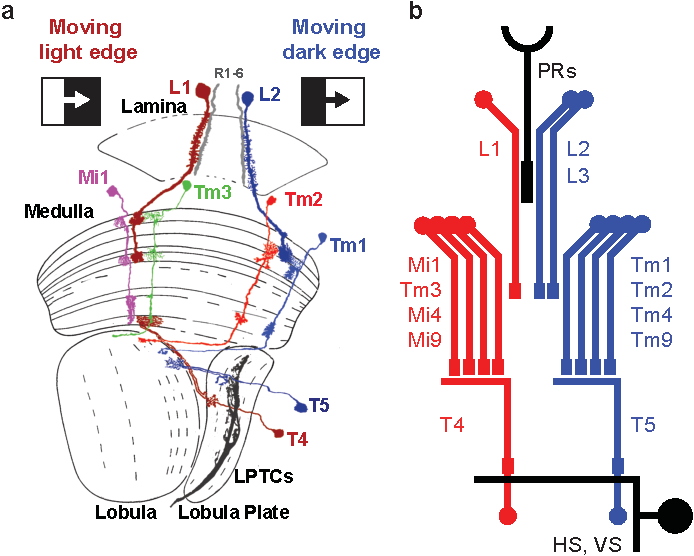
\includegraphics[width=.44\textwidth]{figs/flysetup}
\caption{\small Motion circuits in the fly. (a) Light is detected at the
retina (top) and information is processed
down through different neuropils. Each of the highlighted
neurons is required for motion detection. One circuit 
detects light edges moving over dark backgrounds and another 
dark edges over light backgrounds. (b) Cartoon of
neurons involved in motion detection in the light edge
(red) and dark edge (blue) pathways. 
There are four T4s and four T5s, selective for each
of the four cardinal directions across the retina. This circuit repeats at all
points in space.}
    \label{fig:setup}
    \vskip-10pt
\end{wrapfigure}


The fruit fly \textit{Drosophila} has several advantages for studying the
distributed visual processing that guides perception and
behavior. First, there is a powerful genetic toolbox in fruit flies
that allows researchers to genetically define, manipulate, and monitor
specific classes of neurons \citep{luo:08}. These manipulations
allow specific neurons to be causally connected to
behaviors. Second, the fly has a wealth of visual behaviors,
including regulation of turning and speed, escape, and
courtship \citep{card:08,silies:14,spieth:74}.
Third, the field has identified neuron types that
appear to be making the inferences described above (Fig. 1), including for: 
local motion direction and speed \citep{Maisak:13};
wide-field motion such as rotational
self-motion of the fly about various axes \citep{joesch:08};
looming (approaching) 
dots \citep{devries:12,klapoetke:17}; and 
moving dots \citep{keles:17}. In each case, we
can silence the neurons and observe behavioral deficits. We can also
record activity in these individual neurons and measure their
response properties with well-controlled visual stimuli
\citep{salazar:16}. Thus, these neuron classes act as
handles for understanding how visual inferences are made, and how
neurons extract specific visual features from a spatiotemporally
distributed set of inputs.


\statbackground{}
Statistical theory studies the difficulty of estimation under
various models, and attempts to find optimal estimation
procedures. Such studies usually assume that all of the collected
data are available to construct the estimators. Recent research
has begun to study the problem of statistical estimation in distributed settings, 
as the data can be collected or
stored on multiple machines at different locations. In order to obtain an estimate of some
statistical functional, information needs to be gathered and
aggregated from the multiple locations to form the final
estimate. However, the communication between machines may be
limited. In such a setting, it is important to understand how the
statistical risk of estimation degrades as the communication budget
becomes more constrained.

The so-called CEO problem, first studied in the EE 
community in the context of rate-distortion theory, treats a
similar distributed estimation problem \citep{berger1996ceo,
  viswanathan1997quadratic}. Several later studies
focused on more specific statistical tasks, including mean
estimation, regression, principal eigenspace estimation, and discrete
density estimation \citep{zhang2013information, shamir2014fundamental,
  battey2015distributed, braverman2016communication,
  diakonikolas2017communication, fan2017distributed,
  lee2017communication, shang2017computational}. Most of this 
research treats parametric and discrete models, where the
parameter of interest has finite dimension.  In a nonparametric
setting, the effective dimension of the problem typically grows with
the sample size, and these results no longer apply.
Other results have been obtained on these problems in the normal means
model of nonparametric estimation, which arises naturally when representing an estimator in terms of an
orthogonal
basis \citep{johnstone2002function,tsybakov:2008}.  One
result gives a sharp constrained minimax analysis of nonparametric
regression under quantization constraints \citep{Zhu:18}; another
characterizes lower bounds and achievability for distributed
nonparametric regression \citep{Zhu:18b}. Similar results have been obtained 
using wavelets and Besov spaces \citep{szabo18}.


\project{Parallel channels for local motion detection}
The fly's eye is arranged in a hexagonal lattice of repeated circuit
motifs, with each column of circuitry representing one retinotopic
point in visual space. Each eye consists of an array of ~800 of
these pixels, which together cover approximately one half of visual
space. Two classes of local motion detection cells exist in every
column: T4 cells detect light edges moving across
dark backgrounds and T5 cells detect dark edges moving across
light backgrounds. There are 4 of each class, one for each cardinal
direction, for a total of 8 parallel channels at each point in space
representing motion in two dimensions. Why is the system organized
this way? How are naturalistic motion signals distributed over the 8
channels, and what encoding or decoding advantages does this serve?
Under what conditions are the channels redundant? How would an optimal
observer partition signals among these parallel channels? Could a data-driven 
approach predict or give insight into this encoding scheme?
One approach to begin studying these questions will be to adapt
the classical framework of sparse coding \citep{Olshausen:Field:96}
in a way that represents the neurobiology of the fly's visual system.

\project{Detecting motion flow fields}
When an animal moves or rotates, its
self-motion generates flow fields across its retina. These flow fields
can be used as feedback to control orientation or speed.
In \textit{Drosophila}, some neurons downstream of local motion
detectors have large receptive fields that integrate motion signals
over the retina. They appear selective for specific flow
fields, which correspond to those created by the rotation of
the fly about different axes. These neural signals have been proposed
to be linear filters, matching their weighting for local motion to
specific optical flow fields (``matched filters''). However, it is not
clear whether a linear weighting of local motion estimates is
the best estimate of each field, or whether more complex dendritic
computations could improve encoding. In particular, it is not clear
how these neurons optimally integrate motion signals in the
presence of occlusions or differential velocity fields 
caused by fly translation through space. We will investigate these
issues using methods based on hierarchical sparse coding 
\citep{Yu:2011} and related computational methods for
low-rank decomposition.


\setlength{\columnsep}{10pt}
\begin{wrapfigure}{l}{0.45\textwidth}
\vskip-10pt
\centering
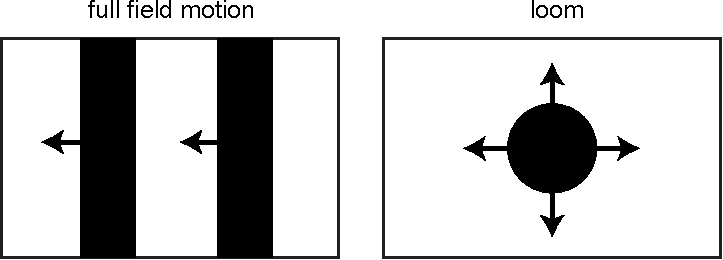
\includegraphics[width=.44\textwidth]{figs/loom}
\caption{\small Global motion and loom generate similar local
motion signals, which must be integrated over space
to distinguish the two stimulus types.}
    \label{fig:loom}
\vskip-20pt
\end{wrapfigure}

\project{Detecting looming stimuli}
Looming stimuli are created by objects as they approach the observer:
the object becomes larger, and if on a collision course,
opposite edges of the object will move in opposite directions on the
retina. Thus, detecting loom requires integrating information over
space, as any local motion detector cannot know if local motion is due
to a looming object or wide-field motion (Fig. 2). Two neuron types in
\textit{Drosophila} have recently been described as loom detectors,
responding selectively as objects grow larger in their receptive
fields. The receptive fields of these cells to local motion have been
characterized, but the relationship between these receptive fields,
the nonlinear computations of these neurons, and the statistics of
natural loom stimuli remain unclear. This is partly due to the
absence of natural statistics on loom stimuli. These loom detectors 
may also use features beyond motion to
detect approaching objects. For instance, a detector might integrate
motion signals with light intensity, since light intensity
is correlated with distance. One might also ask whether the
motion-detecting neurons upstream of the loom-sensitive neurons could
convey information about stimulus features beyond motion
direction and speed. We will abstract loom detection as a statistical
testing problem, building on work such
as \citep{castro:05}. %,huo:06,hc:04}. 
Specifically, for a given object
geometry such as a disk, we will study minimax rates for loom
detection, in terms of the noise level and sparsity of the number of
boundary neuron measurements required. Fast hierarchical algorithms
to achieve the minimax rates will be studied.



